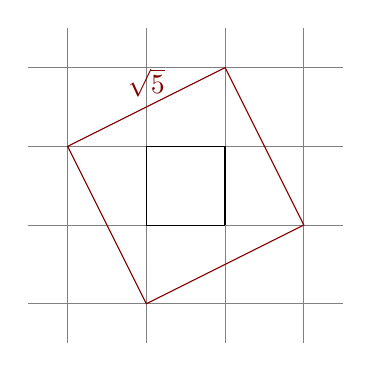
\begin{tikzpicture}
    \draw[gray] (-1.5,-1.5) grid (2.5,2.5);
    \draw[black] (0,0) grid (1,1);
    \draw[red!50!black] (-1,1) -- (1,2) node[midway, above]{$\sqrt{5}$} -- (2,0) -- (0,-1) -- cycle;
    % \node [fill=red,inner sep=1pt,label=below:$X$] (X) at ($ (A)!.5!(B) $) {};
    \end{tikzpicture}